% Options for packages loaded elsewhere
\PassOptionsToPackage{unicode}{hyperref}
\PassOptionsToPackage{hyphens}{url}
%
\documentclass[
]{article}
\usepackage{lmodern}
\usepackage{amssymb,amsmath}
\usepackage{ifxetex,ifluatex}
\ifnum 0\ifxetex 1\fi\ifluatex 1\fi=0 % if pdftex
  \usepackage[T1]{fontenc}
  \usepackage[utf8]{inputenc}
  \usepackage{textcomp} % provide euro and other symbols
\else % if luatex or xetex
  \usepackage{unicode-math}
  \defaultfontfeatures{Scale=MatchLowercase}
  \defaultfontfeatures[\rmfamily]{Ligatures=TeX,Scale=1}
\fi
% Use upquote if available, for straight quotes in verbatim environments
\IfFileExists{upquote.sty}{\usepackage{upquote}}{}
\IfFileExists{microtype.sty}{% use microtype if available
  \usepackage[]{microtype}
  \UseMicrotypeSet[protrusion]{basicmath} % disable protrusion for tt fonts
}{}
\makeatletter
\@ifundefined{KOMAClassName}{% if non-KOMA class
  \IfFileExists{parskip.sty}{%
    \usepackage{parskip}
  }{% else
    \setlength{\parindent}{0pt}
    \setlength{\parskip}{6pt plus 2pt minus 1pt}}
}{% if KOMA class
  \KOMAoptions{parskip=half}}
\makeatother
\usepackage{xcolor}
\IfFileExists{xurl.sty}{\usepackage{xurl}}{} % add URL line breaks if available
\IfFileExists{bookmark.sty}{\usepackage{bookmark}}{\usepackage{hyperref}}
\hypersetup{
  pdftitle={Which Variables help in predicting supermarket revenue? Evidence from Chicago},
  hidelinks,
  pdfcreator={LaTeX via pandoc}}
\urlstyle{same} % disable monospaced font for URLs
\usepackage[margin=1in]{geometry}
\usepackage{graphicx,grffile}
\makeatletter
\def\maxwidth{\ifdim\Gin@nat@width>\linewidth\linewidth\else\Gin@nat@width\fi}
\def\maxheight{\ifdim\Gin@nat@height>\textheight\textheight\else\Gin@nat@height\fi}
\makeatother
% Scale images if necessary, so that they will not overflow the page
% margins by default, and it is still possible to overwrite the defaults
% using explicit options in \includegraphics[width, height, ...]{}
\setkeys{Gin}{width=\maxwidth,height=\maxheight,keepaspectratio}
% Set default figure placement to htbp
\makeatletter
\def\fps@figure{htbp}
\makeatother
\setlength{\emergencystretch}{3em} % prevent overfull lines
\providecommand{\tightlist}{%
  \setlength{\itemsep}{0pt}\setlength{\parskip}{0pt}}
\setcounter{secnumdepth}{-\maxdimen} % remove section numbering

\title{Which Variables help in predicting supermarket revenue? Evidence from
Chicago}
\author{}
\date{\vspace{-2.5em}}

\begin{document}
\maketitle

\hypertarget{introduction}{%
\subsection{Introduction}\label{introduction}}

Location choice is critical to retail organization, due to its effect on
supermarket success (Clarkson, Clarke-Hill, and Robinson 1996). To
choose the outlet location, previous studies have suggested that the
location of supermarkets largely depends on local demographic profile
(Baviera-Puig, Buitrago-Vera, and Escriba-Perez 2016). Our study
considers 45 demographic variables and tries to answer the research
question: what demographic variables are important for predicting the
revenue of supermarkets? We examine which variables make the biggest
impact through an elastic net. This model is chosen because it has shown
to work better than other regularized regressions, such as the least
absolute shrinkage method (LASSO), when several variables are highly
correlated (Zou and Hastie 2005) We assess the best parameters for the
model using k-fold cross validation to further prevent overfitting
(Friedman, Hastie, and Tibshirani 2001). We find that \ldots{} matter
most.

\hypertarget{data}{%
\subsection{Data}\label{data}}

Our research works with a dataset of 45 demographic variables related to
77 supermarkets located around the Chicago area from the year of 1996.
We define demographic data as data that reflects a profile of the
customers; examples of such data included in our dataset are such as
age, sex, income level, race, employment, homeownership, and level of
education. A full description of each variable included can be found in
table 1 of the appendix. Table 2 includes summary statistics. Past
studies have indicated that these variables likely affect the
supermarket turnover. For example, the variable of income has a relation
to food consumption in supermarket (Jones 1997); the variable of gender
may influence the choice of supermarket (Beynon, Moutinho, and Veloutsou
2010); and the variable of race composition may have an impact on
supermarket location(Lamichhane et al. 2013). Our response variable is
yearly total turnover (\$). The demographic data were derived from the
U.S. government's (1990) census for the Chicago metropolitan area. We
scale both the independent and dependent variables as follows:\\
\begin{align*}
\tilde{X} = \frac{X - \mu}{\sqrt{\frac{\sum \boldsymbol{X^2}}{n-1} }}
\end{align*} Where \(\tilde{X}\) is the scaled variable, \(X\) is the
unscaled variable, \(\mu\) is the mean of \(\boldsymbol{X}\), and \(n\)
denotes the sample size. This scaling is done to ensure a fair
interpretation of the model coefficients, as the range of each variable
is different. Table 2 of the appendix shows that several variables are
highly correlated.

\hypertarget{method}{%
\subsection{Method}\label{method}}

In short, our method is using an elastic net, which deals with
overfitting by using a weighted average of the penalty terms applied in
the LASSO and ridge regression. Before we explain the elastic net, let's
consider the standard linear regression model: \begin{align*}
    \hat{\boldsymbol{y}} = \mathbf{X}\boldsymbol{\hat{\beta}}
\end{align*} In which \(\hat{\boldsymbol{y}}\) is an n x 1 column vector
of the predicted response variable, \(\mathbf{X}\) is an n x (p+1)
matrix with n observations of p predictor variables and the intercept.
\(\boldsymbol{\hat{\beta}}\) is an (1 + p) x 1 column vector of the
estimated coefficients for true parameter \(\boldsymbol{{\beta}}\) of
the intercept and \(p\) predictor variables. The standard method for
finding the optimal \(\boldsymbol{\beta}\) is the ordinary least squared
(OLS) method that minimizes the sum of squared error between the
predicted and observed response variables \(\hat{\boldsymbol{y}}\) and
\({\boldsymbol{y}}\). Thus the following loss function is minimized:
\begin{align*}
    L(\boldsymbol{\beta}) = (\boldsymbol{y} - \mathbf{X}\boldsymbol{\beta})^T(\boldsymbol{y} - \mathbf{X}\boldsymbol{\beta})
\end{align*} The problem with using this method is that it is prone to
overfitting (Friedman, Hastie, and Tibshirani 2001). This is because
when applied to a training set, it often overestimates the effect of
certain variables. In order to solve this, a new set of methods emerged
called regularized regression, in which penalty terms are added to the
above loss function in order to shrink the \(\boldsymbol{\beta}\).
Elastic net is a regularized regression that combines two penalty terms.
\begin{align*}
    P_1(\boldsymbol{\beta}) = \lambda \sum_{i=1}^{p} \vert \beta_i \vert \hspace{35pt} P_2(\boldsymbol{\beta}) = \lambda \boldsymbol{\beta}^T\boldsymbol{\beta}
\end{align*} In which \(P_1, P_2\) are the two penalty terms, and
\(\lambda\) is a constant parameter that determines their size. The
\(P_1\) is the sum of the absolute value of the coefficients, and is
used in the so-called LASSO method (Tibshirani 1996). When this penalty
term is used, coefficients are continuously reduced, or removed
completely.

But using just this penalty term has several downsides; it performs less
well when \(p \geq n\), and when several variables are highly correlated
(Zou and Hastie 2005) . Zhou and Hastie (2005) show that in these
circumstances, the elastic net performs better than the Lasso, by adding
a second penalty term, \(P_2\). This is the same penalty used in a ridge
regression (Hoerl and Kennard 1970). Elastic net then determines the
weight between the two penalty terms, using the constant parameter
\(\alpha\). Given the high correlation between several of the variables
in our dataset, it seems appropriate to use the elastic net. This gives
the following loss function for an elastic net: \begin{align*}
    L(\boldsymbol{\beta}) = (\boldsymbol{y} - \mathbf{X}\boldsymbol{\beta})^T(\boldsymbol{y} - \mathbf{X}\boldsymbol{\beta}) + \lambda \alpha \sum_{i=1}^{p} \vert \beta_i \vert + \lambda (1-\alpha) \boldsymbol{\beta}^T\boldsymbol{\beta}
\end{align*} In order to find the \(\boldsymbol{\beta}\) at which
\(L(\boldsymbol{\beta})\) is minimized, we use the majorize-minimization
algorithm (MM). We use the following majorization function:
\begin{align*}
    L(\boldsymbol{\beta})=\frac{1}{2}\boldsymbol{\beta}^T(\mathbf{A})\boldsymbol{\beta} - n^{-1}\boldsymbol{\beta}^T\mathbf{X}^T\boldsymbol{y} + c \\
    \mathbf{A} = n^{-1}\mathbf{X}^T\mathbf{X} + \lambda(1+\alpha)I + \lambda \alpha \mathbf{D}\\
    \mathbf{D} = \begin{bmatrix}
    \frac{1}{max(\beta_1, \epsilon)} & & \\
    & \ddots & \\
    & & \frac{1}{max(\beta_p, \epsilon)} \\
  \end{bmatrix} \\
   c = \frac{1}{2n}\boldsymbol{y}^T\boldsymbol{y} + \frac{1}{2}\lambda\alpha  \sum_{i=1}^{p} \vert \beta_i \vert
\end{align*} We then find the \(\boldsymbol{\beta}\) for which this
function is minimized through stepwise updating the
\(\boldsymbol{\beta}\). This happens by solving the following:
\begin{align*}
   \hat{\boldsymbol{\beta_k}} = (\mathbf{A})^{-1}n^{-1}\mathbf{X}^T\boldsymbol{y}
\end{align*} Where \(\hat{\boldsymbol{\beta_k}}\) is the estimated
\(\boldsymbol{\beta}\) at step k. This stepwise updating continues until
the next set of \(\boldsymbol{\beta}\) does not improve by more than
\(\epsilon\). To find the \(\lambda\) and \(\alpha\) for our elastic
net, we use K-fold cross validation. In this method, the dataset is
split into \(K\) random samples. One of the samples is picked as the
validation test, and the \(\boldsymbol{\beta}\) are determined based on
the remaining K-1 samples. This then happens K times, until each of the
samples is used as a validation test. For each iteration, we calculate
the root mean squared error, and then the average RMSE across the K
validations. \begin{align*}
    RMSE = \sqrt{ \frac{1}{n} \sum_{i=1}^{n} (\hat{\boldsymbol{y}} - \boldsymbol{y})^2 } \hspace{35pt} \text{Average RMSE} = \frac{1}{K}\sum_{i=1}^{K} RMSE_i 
\end{align*}\\
In which \(RMSE_i\) is the RMSE of the validation on sample \(i\). Our
metric for picking the \(\lambda\) and \(\alpha\) is the lowest average
RMSE. The process of finding this metric process is visualized below for
K = 4.

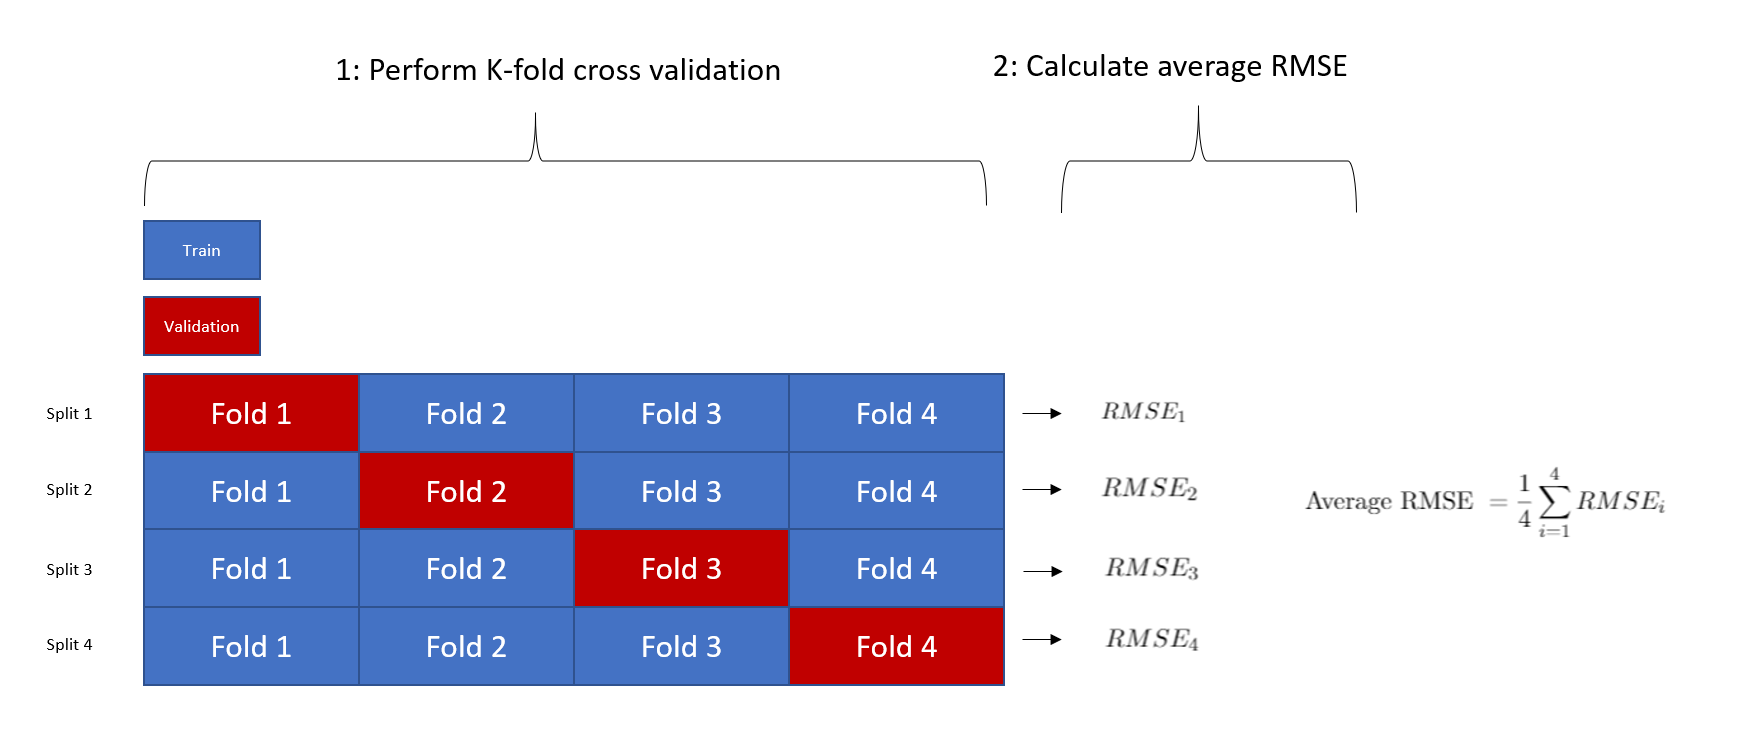
\includegraphics[]{kfold.PNG}

Using K-fold cross validation to pick the ideal \(\lambda, \alpha\)
reduces the likelihood of overfitting, since the parameters are not just
based on one random sample, but on multiple, reducing the likelihood
that features from one sample dominate when predicting. We fold our
sample 10 times - this allows us to use a lot of different folds,
without becoming computationally too expensive. We use RMSE to measure
the error between our prediction and the actual values. The squaring of
these errors ensures that larger errors contribute more, which reduces
the chance of our model making large mistakes. When looking for our
ideal \(\lambda, \alpha\), we evaluate all possible combinations between
the two following sets: \begin{align*}
    \alpha = [0,0.1,0.2...1] \hspace{35pt} x = \{x   \vert -2 \leq x \leq 10\} , \lambda = 10^x\\
\end{align*}

\hypertarget{results}{%
\subsection{Results}\label{results}}

\hypertarget{appendix}{%
\subsection{Appendix}\label{appendix}}

\hypertarget{table-a-summary-statistics}{%
\subsubsection{Table A: Summary
Statistics}\label{table-a-summary-statistics}}

\begin{table}[!htbp] \centering 
\tiny
\begin{tabular}{@{\extracolsep{5pt}}lccccccc} 
\\[-1.8ex]\hline 
\hline \\[-1.8ex] 
Statistic & \multicolumn{1}{c}{N} & \multicolumn{1}{c}{Mean} & \multicolumn{1}{c}{St. Dev.} & \multicolumn{1}{c}{Min} & \multicolumn{1}{c}{Pctl(25)} & \multicolumn{1}{c}{Pctl(75)} & \multicolumn{1}{c}{Max} \\ 
\hline \\[-1.8ex] 
GROCERY\_sum & 77 & 7,341,015.000 & 2,341,073.000 & 1,423,582.000 & 5,778,987.000 & 9,022,599.000 & 13,165,586.000 \\ 
AGE9 & 77 & 0.138 & 0.025 & 0.046 & 0.121 & 0.151 & 0.193 \\ 
AGE60 & 77 & 0.173 & 0.063 & 0.058 & 0.122 & 0.214 & 0.307 \\ 
ETHNIC & 77 & 0.160 & 0.193 & 0.024 & 0.044 & 0.188 & 0.996 \\ 
EDUC & 77 & 0.227 & 0.114 & 0.050 & 0.146 & 0.284 & 0.528 \\ 
NOCAR & 77 & 0.113 & 0.132 & 0.012 & 0.025 & 0.144 & 0.551 \\ 
INCOME & 77 & 10.616 & 0.293 & 9.867 & 10.414 & 10.797 & 11.236 \\ 
INCSIGMA & 77 & 24,840.880 & 2,295.236 & 20,359.560 & 23,488.270 & 26,458.280 & 30,276.640 \\ 
HSIZEAVG & 77 & 2.665 & 0.263 & 1.554 & 2.543 & 2.790 & 3.309 \\ 
HSIZE1 & 77 & 0.245 & 0.083 & 0.122 & 0.200 & 0.269 & 0.614 \\ 
HSIZE2 & 77 & 0.309 & 0.031 & 0.219 & 0.290 & 0.333 & 0.369 \\ 
HSIZE34 & 77 & 0.330 & 0.060 & 0.092 & 0.306 & 0.367 & 0.446 \\ 
HSIZE567 & 77 & 0.116 & 0.031 & 0.014 & 0.098 & 0.132 & 0.216 \\ 
HH3PLUS & 77 & 0.446 & 0.083 & 0.106 & 0.405 & 0.490 & 0.650 \\ 
HH4PLUS & 77 & 0.274 & 0.063 & 0.041 & 0.241 & 0.305 & 0.443 \\ 
HHSINGLE & 77 & 0.245 & 0.083 & 0.122 & 0.200 & 0.269 & 0.614 \\ 
HHLARGE & 77 & 0.116 & 0.031 & 0.014 & 0.098 & 0.132 & 0.216 \\ 
WORKWOM & 77 & 0.358 & 0.053 & 0.244 & 0.312 & 0.402 & 0.472 \\ 
SINHOUSE & 77 & 0.548 & 0.216 & 0.017 & 0.517 & 0.706 & 0.822 \\ 
DENSITY & 77 & 0.001 & 0.001 & 0.0001 & 0.0004 & 0.001 & 0.005 \\ 
HVAL150 & 77 & 0.349 & 0.246 & 0.003 & 0.123 & 0.534 & 0.917 \\ 
HVAL200 & 77 & 0.186 & 0.186 & 0.001 & 0.043 & 0.268 & 0.781 \\ 
HVALMEAN & 77 & 147.907 & 47.534 & 64.348 & 108.924 & 179.072 & 267.390 \\ 
SINGLE & 77 & 0.280 & 0.068 & 0.203 & 0.242 & 0.286 & 0.593 \\ 
RETIRED & 77 & 0.150 & 0.051 & 0.056 & 0.109 & 0.188 & 0.236 \\ 
UNEMP & 77 & 0.182 & 0.023 & 0.142 & 0.166 & 0.195 & 0.245 \\ 
WRKCH5 & 77 & 0.056 & 0.020 & 0.024 & 0.041 & 0.070 & 0.118 \\ 
WRKCH17 & 77 & 0.124 & 0.029 & 0.041 & 0.103 & 0.144 & 0.198 \\ 
NWRKCH5 & 77 & 0.084 & 0.028 & 0.030 & 0.064 & 0.101 & 0.169 \\ 
NWRKCH17 & 77 & 0.070 & 0.021 & 0.018 & 0.059 & 0.082 & 0.122 \\ 
WRKCH & 77 & 0.180 & 0.044 & 0.071 & 0.149 & 0.214 & 0.293 \\ 
NWRKCH & 77 & 0.154 & 0.043 & 0.048 & 0.123 & 0.183 & 0.250 \\ 
WRKWCH & 77 & 0.055 & 0.020 & 0.024 & 0.041 & 0.069 & 0.115 \\ 
WRKWNCH & 77 & 0.258 & 0.044 & 0.157 & 0.227 & 0.282 & 0.460 \\ 
TELEPHN & 77 & 0.977 & 0.029 & 0.839 & 0.976 & 0.993 & 0.998 \\ 
MORTGAGE & 77 & 0.710 & 0.147 & 0.443 & 0.617 & 0.826 & 0.960 \\ 
NWHITE & 77 & 0.204 & 0.194 & 0.035 & 0.091 & 0.205 & 0.995 \\ 
POVERTY & 77 & 0.058 & 0.045 & 0.014 & 0.027 & 0.076 & 0.213 \\ 
SHPCONS & 77 & 0.082 & 0.062 & 0.019 & 0.037 & 0.115 & 0.279 \\ 
SHPHURR & 77 & 0.153 & 0.059 & 0.026 & 0.110 & 0.191 & 0.286 \\ 
SHPAVID & 77 & 0.189 & 0.043 & 0.061 & 0.161 & 0.220 & 0.310 \\ 
SHPKSTR & 77 & 0.284 & 0.066 & 0.184 & 0.232 & 0.330 & 0.558 \\ 
SHPUNFT & 77 & 0.246 & 0.055 & 0.145 & 0.197 & 0.291 & 0.391 \\ 
SHPBIRD & 77 & 0.046 & 0.025 & 0.004 & 0.025 & 0.064 & 0.105 \\ 
SHOPINDX & 77 & 0.736 & 0.246 & 0.00000 & 0.730 & 0.890 & 0.986 \\ 
\hline \\[-1.8ex] 
\end{tabular} 
\end{table}

\hypertarget{table-b-correlation-matrix}{%
\subsubsection{Table B: Correlation
Matrix}\label{table-b-correlation-matrix}}

\textbackslash begin\{table\}{[}!htbp{]} \centering 

\caption{} 
  \label{}

\textbackslash begin\{tabular\}\{@\{\extracolsep{5pt}\} cccc\}
\textbackslash{[}-1.8ex{]}\hline  \hline \textbackslash{[}-1.8ex{]} \&
Var1 \& Var2 \& Freq \textbackslash{} \hline \textbackslash{[}-1.8ex{]}
1 \& HSIZE1 \& HSIZE34 \& \[-$0.966$ \\ 
2 & HSIZEAVG & HSIZE1 & \]-\(0.908\) \textbackslash{} 3 \& HH4PLUS \&
HHSINGLE \& \[-$0.887$ \\ 
4 & MORTGAGE & SHPBIRD & \]-\(0.869\) \textbackslash{} 5 \& SINHOUSE \&
SINGLE \& \[-$0.862$ \\ 
6 & WORKWOM & RETIRED & \]-\(0.859\) \textbackslash{} 7 \& NOCAR \&
INCOME \& \[-$0.835$ \\ 
8 & SHPCONS & SHPHURR & \]-\(0.810\) \textbackslash{} 9 \& HHLARGE \&
WRKWNCH \& \[-$0.800$ \\ 
10 & HHSINGLE & SINHOUSE & \]-\(0.798\) \textbackslash{} 11 \& HSIZE2 \&
UNEMP \& \[-$0.775$ \\ 
12 & TELEPHN & NWHITE & \]-\(0.761\) \textbackslash{} 13 \& RETIRED \&
WRKCH17 \& \[-$0.727$ \\ 
14 & SINGLE & TELEPHN & \]-\(0.726\) \textbackslash{} 15 \& UNEMP \&
TELEPHN \& \[-$0.726$ \\ 
16 & ETHNIC & INCOME & \]-\(0.720\) \textbackslash{} 17 \& AGE9 \& AGE60
\& \$-\$0.700 \textbackslash{} 18 \& EDUC \& INCSIGMA \& \(0.717\)
\textbackslash{} 19 \& WRKCH5 \& NWRKCH5 \& \(0.745\) \textbackslash{}
20 \& WRKCH17 \& NWRKCH5 \& \(0.748\) \textbackslash{} 21 \& WRKCH \&
NWRKCH \& \(0.749\) \textbackslash{} 22 \& INCSIGMA \& HVAL150 \&
\(0.779\) \textbackslash{} 23 \& SHPHURR \& SHOPINDX \& \(0.779\)
\textbackslash{} 24 \& NWRKCH \& SHPHURR \& \(0.790\) \textbackslash{}
25 \& INCOME \& INCSIGMA \& \(0.796\) \textbackslash{} 26 \& HSIZE567 \&
HH3PLUS \& \(0.836\) \textbackslash{} 27 \& NWRKCH17 \& NWRKCH \&
\(0.838\) \textbackslash{} 28 \& NWHITE \& POVERTY \& \(0.841\)
\textbackslash{} 29 \& NWRKCH5 \& WRKCH \& \(0.841\) \textbackslash{} 30
\& AGE60 \& RETIRED \& \(0.877\) \textbackslash{} 31 \& HVAL150 \&
HVAL200 \& \(0.928\) \textbackslash{} 32 \& HVAL200 \& HVALMEAN \&
\(0.943\) \textbackslash{} 33 \& HSIZE34 \& HH3PLUS \& \(0.959\)
\textbackslash{} 34 \& HH3PLUS \& HH4PLUS \& \(0.990\) \textbackslash{}
35 \& POVERTY \& SHPCONS \& \(0.997\) \textbackslash{}
\hline \textbackslash{[}-1.8ex{]} \textbackslash end\{tabular\}
\textbackslash end\{table\}

\hypertarget{Reference}{%
\subsection*{Reference}\label{Reference}}
\addcontentsline{toc}{subsection}{Reference}

\hypertarget{refs}{}
\leavevmode\hypertarget{ref-baviera2016geomarketing}{}%
Baviera-Puig, Amparo, Juan Buitrago-Vera, and Carmen Escriba-Perez.
2016. ``Geomarketing Models in Supermarket Location Strategies.''
\emph{Journal of Business Economics and Management} 17 (6): 1205--21.

\leavevmode\hypertarget{ref-beynon2010gender}{}%
Beynon, Malcolm J, Luiz Moutinho, and Cleopatra Veloutsou. 2010.
``Gender Differences in Supermarket Choice.'' \emph{European Journal of
Marketing}.

\leavevmode\hypertarget{ref-clarkson1996uk}{}%
Clarkson, Richard M, Colin M Clarke-Hill, and Terry Robinson. 1996. ``UK
Supermarket Location Assessment.'' \emph{International Journal of Retail
\& Distribution Management}.

\leavevmode\hypertarget{ref-friedman2001elements}{}%
Friedman, Jerome, Trevor Hastie, and Robert Tibshirani. 2001. \emph{The
Elements of Statistical Learning}. Vol. 1. 10. Springer series in
statistics New York.

\leavevmode\hypertarget{ref-hoerl1970ridge}{}%
Hoerl, Arthur E, and Robert W Kennard. 1970. ``Ridge Regression: Biased
Estimation for Nonorthogonal Problems.'' \emph{Technometrics} 12 (1):
55--67.

\leavevmode\hypertarget{ref-jones1997analysis}{}%
Jones, Eugene. 1997. ``An Analysis of Consumer Food Shopping Behavior
Using Supermarket Scanner Data: Differences by Income and Location.''
\emph{American Journal of Agricultural Economics} 79 (5): 1437--43.

\leavevmode\hypertarget{ref-lamichhane2013spatial}{}%
Lamichhane, Archana P, Joshua Warren, Robin Puett, Dwayne E Porter,
Matteo Bottai, Elizabeth J Mayer-Davis, and Angela D Liese. 2013.
``Spatial Patterning of Supermarkets and Fast Food Outlets with Respect
to Neighborhood Characteristics.'' \emph{Health \& Place} 23: 157--64.

\leavevmode\hypertarget{ref-tibshirani1996regression}{}%
Tibshirani, Robert. 1996. ``Regression Shrinkage and Selection via the
Lasso.'' \emph{Journal of the Royal Statistical Society: Series B
(Methodological)} 58 (1): 267--88.

\leavevmode\hypertarget{ref-zou2005regularization}{}%
Zou, Hui, and Trevor Hastie. 2005. ``Regularization and Variable
Selection via the Elastic Net.'' \emph{Journal of the Royal Statistical
Society: Series B (Statistical Methodology)} 67 (2): 301--20.

\end{document}
